\documentclass[11pt,twoside]{book}

\newcommand{\utilchap}{\chapter}
\newcommand{\utilsect}{\section}
\newcommand{\textchap}{chapter}

%% include commands for bios, titles etc used in multiple documents
%%
% $Date$
% $Revision$
% $Author$

%%%%%%%%%%%%%%%%%%%%%%%%%%%%%%%%%%%%%%%%%%%%%%%%%%%%%%%%%%%%%%%%%%%%%%%%%%%%%%%%%%%%%%%%%%%%%%%%%%%
%                                                                                                 %
% The mathematical style of these documents follows                                               %
%                                                                                                 %
% A. Thompson and B.N. Taylor. The NIST Guide for the Use of the International System of Units.   %
%    NIST Special Publication 881, 2008.                                                          %
%                                                                                                 %
% http://www.nist.gov/pml/pubs/sp811/index.cfm                                                    %
%                                                                                                 %
%%%%%%%%%%%%%%%%%%%%%%%%%%%%%%%%%%%%%%%%%%%%%%%%%%%%%%%%%%%%%%%%%%%%%%%%%%%%%%%%%%%%%%%%%%%%%%%%%%%

% Packages which force the use of better TeX coding
% Mostly from http://tex.stackexchange.com/q/19264
%%\RequirePackage[l2tabu, orthodox]{nag}
%%\usepackage{fixltx2e}
%\usepackage{isomath} % Disabled for the moment because it changes the syntax for bold and roman Greek math symbols
%%\usepackage[all,warning]{onlyamsmath}
%\usepackage{strict} % Commented out for now because it is uncommon. A copy of style.sty is in Manuals/LaTeX_Style_Files/.

\usepackage{times,mathptmx}
\usepackage[pdftex]{graphicx}
\usepackage{tabularx}
\usepackage{multirow}
\usepackage{pdfsync}
\usepackage{tikz}
\usepackage{pgfplots}
%\pgfplotsset{compat=1.7}
\usepackage{tocloft}
\usepackage{color}
\usepackage{amsmath}
\definecolor{linknavy}{rgb}{0,0,0.50196}
\definecolor{linkred}{rgb}{1,0,0}
\definecolor{linkblue}{rgb}{0,0,1}
\usepackage{float}
\usepackage{caption}
\usepackage{graphpap}
\usepackage{rotating}
\usepackage{geometry}
\usepackage{relsize}
\usepackage{longtable}
\usepackage{lscape}
\usepackage{amssymb}
\usepackage{makeidx} % Create index at end of document
\usepackage[nottoc,notlof,notlot]{tocbibind} % Put the bibliography and index in the ToC
\usepackage{lastpage} % Automatic last page number reference.
\usepackage[T1]{fontenc}
\usepackage{enumerate}
\usepackage{upquote}
\usepackage{moreverb}
\usepackage{morefloats}

% Smokeview Version String
\newcommand{\smvversion}{6.5.0}

\newcommand{\nopart}{\expandafter\def\csname Parent-1\endcsname{}} % To fix table of contents in pdf.
\newcommand{\ct}{\tt\small} % eventually will be deprecated due to http://www.tex.ac.uk/cgi-bin/texfaq2html?label=2letterfontcmd
\newcommand{\textct}[1]{\texttt{\small #1}}

\usepackage{tocstyle} % Fix table of contents sections from overlapping section titles
\usetocstyle{standard}
\usepackage{siunitx}
\sisetup{
    detect-all = true,
    input-decimal-markers = {.},
    input-ignore = {,},
    inter-unit-product = \ensuremath{{}\cdot{}},
    multi-part-units = repeat,
    number-unit-product = \text{~},
    per-mode = fraction,
    separate-uncertainty = true,
}

\usepackage{listings}
\usepackage{textcomp}
\definecolor{lbcolor}{rgb}{0.96,0.96,0.96}
\lstset{
    %backgroundcolor=\color{lbcolor},
    tabsize=4,
    rulecolor=,
    language=Fortran,
        basicstyle=\footnotesize\ttfamily,
        upquote=true,
        aboveskip={\baselineskip},
        belowskip={\baselineskip},
        columns=fixed,
        extendedchars=true,
        breaklines=true,
        breakatwhitespace=true,
        frame=none,
        showtabs=false,
        showspaces=false,
        showstringspaces=false,
        identifierstyle=\ttfamily,
        keywordstyle=\color[rgb]{0,0,0},
        commentstyle=\color[rgb]{0,0,0},
        stringstyle=\color[rgb]{0,0,0},
}

\usepackage{xr-hyper}
\usepackage[pdftex,
        colorlinks=true,
        urlcolor=linkblue,     % \href{...}{...} external (URL)
        citecolor=linkred,     % citation number colors
        linkcolor=linknavy,    % \ref{...} and \pageref{...}
        pdfproducer={pdflatex},
        pagebackref,
        pdfpagemode=UseNone,
        bookmarksopen=true,
        plainpages=false,
        verbose]{hyperref}

% The Following commented code makes the ``Draft'' watermark on each page.
%\usepackage{eso-pic}
%\usepackage{type1cm}
%\makeatletter
%   \AddToShipoutPicture{
%     \setlength{\@tempdimb}{.5\paperwidth}
%     \setlength{\@tempdimc}{.5\paperheight}
%     \setlength{\unitlength}{1pt}
%     \put(\strip@pt\@tempdimb,\strip@pt\@tempdimc){
%     \makebox(0,0){\rotatebox{45}{\textcolor[gray]{0.75}{\fontsize{8cm}\selectfont{RC6}}}}}
% }
%\makeatother

\setlength{\textwidth}{6.5in}
\setlength{\textheight}{9.0in}
\setlength{\topmargin}{0.in}
\setlength{\headheight}{0.in}
\setlength{\headsep}{0.in}
\setlength{\parindent}{0.25in}
\setlength{\oddsidemargin}{0.0in}
\setlength{\evensidemargin}{0.0in}
\setlength{\leftmargini}{\parindent} % Controls the indenting of the "bullets" in a list
\setlength{\cftsecnumwidth}{0.45in}
\setlength{\cftsubsecnumwidth}{0.5in}
\setlength{\cftfignumwidth}{0.45in}
\setlength{\cfttabnumwidth}{0.45in}

\newcommand{\authortitlesigs}
{
\begin{flushright}
Kevin McGrattan \\
Simo Hostikka \\
Randall McDermott \\
Jason Floyd \\
Craig Weinschenk \\
Kristopher Overholt
\end{flushright}
}

\newcommand{\logosigs}{
\begin{minipage}[b]{6.5in}
\parbox[b]{3.5in}{

\includegraphics[width=1.3in]{../Bibliography/VTT_BLACK_L} \\
VTT Technical Research Centre of Finland}
\hfill
\parbox[b]{3in}{\flushright{
\includegraphics[width=2.in]{../Bibliography/nistident_flright_vec}}}
\end{minipage}
}

\newcommand{\authorsigs}
{
\begin{flushright}
Kevin McGrattan \\
Randall McDermott \\
{\em Fire Research Division \\
Engineering Laboratory \\
Gaithersburg, Maryland, USA} \\[.1in]
Simo Hostikka \\
{\em Aalto University \\
Espoo, Finland} \\[.1in]
Jason Floyd \\
Craig Weinschenk \\
{\em Jensen Hughes \\
Baltimore, Maryland, USA}\\[.1in]
Kristopher Overholt \\
{\em Continuum Analytics \\
Austin, Texas, USA}
\end{flushright}
}

\newcommand{\titlesigs}
{
\small
\begin{flushright}
U.S. Department of Commerce \\
{\em Wilbur L. Ross, Jr., Secretary} \\
\hspace{1in} \\
National Institute of Standards and Technology \\
{\em Kent Rochford, Acting Under Secretary of Commerce for Standards and Technology and Acting NIST Director}
\end{flushright}
}


\newcommand{\disclaimer}[1]{
\begin{minipage}[t][8in][s]{6.5in}
\fontsize{10}{12}\selectfont
\flushright{Certain commercial entities, equipment, or materials may be identified in this \\
document in order to describe an experimental procedure or concept adequately. \\
Such identification is not intended to imply recommendation or endorsement by the \\
National Institute of Standards and Technology, nor is it intended to imply that the \\
entities, materials, or equipment are necessarily the best available for the purpose.\\
}

\vspace{3in}

\large
\flushright{\bf National Institute of Standards and Technology Special Publication #1 \\
Natl.~Inst.~Stand.~Technol.~Spec.~Publ.~#1, \pageref{LastPage} pages (October 2013) \\
CODEN: NSPUE2 }

\vfill

\hspace{1in}

\end{minipage}
}



\newcommand{\gforneybio}
{
\item[Glenn Forney] is a computer scientist at the Engineering Laboratory of NIST.  He received a
bachelor of science degree in mathematics from Salisbury State College and a master of
science and a doctorate in mathematics from Clemson University.  He joined NIST
in 1986 (then the National Bureau of Standards) and has since worked on developing tools that
provide a better understanding of fire phenomena, most notably Smokeview, a software tool for visualizing
Fire Dynamics Simulator data.
}

\newcommand{\smvoverview}
{
This guide is part of a three volume set of companion documents describing how to use Smokeview
in Volume I, the Smokeview User's Guide~\cite{Smokeview_Users_Guide}, describing technical details of how the visualizations are performed in Volume II, the Smokeview Technical Reference Guide~\cite{Smokeview_Tech_Guide}, and presents example cases
verifying the various visualization capabilities of Smokeview in Volume III, the Smokeview Verification Guide~\cite{Smokeview_Verification_Guide}.  Details on the use and technical background of the Fire Dynamics Simulator is contained in the FDS User's~\cite{FDS_Users_Guide} and Technical reference guide~\cite{FDS_Math_Guide}
respectively.
}

% commands to use for "official" cover and title pages
% see smokeview verification guide to see how they are used

\newcommand{\headerA}[1]{
\begin{flushright}
\fontsize{20}{24}\selectfont
\bf{NIST Special Publication #1}
\end{flushright}
}


\newcommand{\headerB}[1]{
\begin{flushright}
\fontsize{28}{33.6}\selectfont
\bf{#1}
\end{flushright}
}

\newcommand{\headerC}[1]{
\vspace{.15in}
\begin{flushright}
\fontsize{12}{14}\selectfont
#1
\end{flushright}
}

\newcommand{\headerD}[1]{
\begin{flushright}
\fontsize{12}{14}\selectfont
http://dx.doi.org/10.6028/NIST.SP.#1
\end{flushright}
}



\newcommand{\dod}[2]{\frac{\partial #1}{\partial #2}}
\newcommand{\DoD}[2]{\frac{\mathrm{D} #1}{\mathrm{D} #2}}
\newcommand{\dsods}[2]{\frac{\partial^2 #1}{\partial #2^2}}
\renewcommand{\d}{\,\mathrm{d}}
\newcommand{\dx}{\delta x}
\newcommand{\dy}{\delta y}
\newcommand{\dz}{\delta z}
\newcommand{\degF}{$^\circ$F}
\newcommand{\degC}{$^\circ$C}
\newcommand{\x}{x}
\newcommand{\y}{y}
\newcommand{\z}{z}
\newcommand{\dt}{\delta t}
\newcommand{\dn}{\delta n}
\newcommand{\cH}{H}
\newcommand{\hu}{u}
\newcommand{\hv}{v}
\newcommand{\hw}{w}
\newcommand{\la}{\lambda}
\newcommand{\bO}{{\Omega}}
\newcommand{\bo}{{\mathbf{\omega}}}
\newcommand{\btau}{\mathbf{\tau}}
\newcommand{\bdelta}{{\mathbf{\delta}}}
\newcommand{\sumyw}{\sum (Y_\alpha/W_\alpha)}
\newcommand{\oW}{\overline{W}}
\newcommand{\om}{\ensuremath{\omega}}
\newcommand{\omx}{\omega_x}
\newcommand{\omy}{\omega_y}
\newcommand{\omz}{\omega_z}
\newcommand{\erf}{\hbox{erf}}
\newcommand{\erfc}{\hbox{erfc}}
\newcommand{\bF}{{\mathbf{F}}}
\newcommand{\bG}{{\mathbf{G}}}
\newcommand{\bof}{{\mathbf{f}}}
\newcommand{\bq}{{\mathbf{q}}}
\newcommand{\br}{{\mathbf{r}}}
\newcommand{\bu}{{\mathbf{u}}}
\newcommand{\bx}{{\mathbf{x}}}
\newcommand{\bk}{{\mathbf{k}}}
\newcommand{\bv}{{\mathbf{v}}}
\newcommand{\bg}{{\mathbf{g}}}
\newcommand{\bn}{{\mathbf{n}}}
\newcommand{\bS}{{\mathbf{S}}}
\newcommand{\bW}{\overline{W}}
\newcommand{\dS}{d{\mathbf{S}}}
\newcommand{\bs}{{\mathbf{s}}}
\newcommand{\bI}{{\mathbf{I}}}
\newcommand{\hp}{H}
\newcommand{\trho}{\tilde{\rho}}
\newcommand{\dph}{{\delta\phi}}
\newcommand{\dth}{{\delta\theta}}
\newcommand{\tp}{\tilde{p}}
\newcommand{\bp}{\overline{p}}
\newcommand{\dQ}{\dot{Q}}
\newcommand{\dq}{\dot{q}}
\newcommand{\dbq}{\dot{\mathbf{q}}}
\newcommand{\dm}{\dot{m}}
\newcommand{\ha}{\frac{1}{2}}
\newcommand{\ft}{\frac{4}{3}}
\newcommand{\ot}{\frac{1}{3}}
\newcommand{\fofi}{\frac{4}{5}}
\newcommand{\of}{\frac{1}{4}}
\newcommand{\twth}{\frac{2}{3}}
\newcommand{\R}{R}
\newcommand{\be}{\begin{equation}}
\newcommand{\ee}{\end{equation}}
\newcommand{\RE}{\hbox{Re}}
\newcommand{\LE}{\hbox{Le}}
\newcommand{\PR}{\hbox{Pr}}
\newcommand{\PE}{\hbox{Pe}}
\newcommand{\NU}{\hbox{Nu}}
\newcommand{\SC}{\hbox{Sc}}
\newcommand{\SH}{\hbox{Sh}}
\newcommand{\WE}{\hbox{We}}
\newcommand{\COTWO}{\text{\tiny \hbox{CO}$_2$}}
\newcommand{\HTWOO}{\text{\tiny \hbox{H}$_2$\hbox{O}}}
\newcommand{\OTWO}{\text{\tiny \hbox{O}$_2$}}
\newcommand{\NTWO}{\text{\tiny \hbox{N}$_2$}}
\newcommand{\CO}{\text{\tiny \hbox{CO}}}
\newcommand{\F}{\text{\tiny \hbox{F}}}
\newcommand{\C}{\text{\tiny \hbox{C}}}
\newcommand{\Hy}{\text{\tiny \hbox{H}}}
\newcommand{\So}{\text{\tiny \hbox{S}}}
\newcommand{\M}{\text{\tiny \hbox{M}}}
\newcommand{\xx}{\text{\tiny \hbox{x}}}
\newcommand{\yy}{\text{\tiny \hbox{y}}}
\newcommand{\zz}{\text{\tiny \hbox{z}}}
\newcommand{\smvlines}{135~000}

\newcommand{\calH}{\mathcal{H}}
\newcommand{\calR}{\mathcal{R}}

\newcommand{\dif}{\mathrm{d}}
\newcommand{\Div}{\nabla\cdot}
\newcommand{\D}{\mbox{D}}
\newcommand{\mhalf}{\mbox{$\frac{1}{2}$}}
\newcommand{\thalf}{\mbox{\tiny $\frac{1}{2}$}}
\newcommand{\tripleprime}{{\prime\prime\prime}}
\newcommand{\ppp}{{\prime\prime\prime}}
\newcommand{\pp}{{\prime\prime}}

\newcommand{\superscript}[1]{\ensuremath{^{\textrm{\tiny #1}}}}
\newcommand{\subscript}[1]{\ensuremath{_{\textrm{\tiny #1}}}}

\newcommand{\rb}[1]{\raisebox{1.5ex}[0pt]{#1}}

\newcommand{\Ra}{$\Rightarrow$}
\newcommand{\hhref}[1]{\href{#1}{{\tt #1}}}
\newcommand{\fdsinput}[1]{{\scriptsize\verbatiminput{../../Verification/Visualization/#1}}}

\definecolor{AQUAMARINE}{rgb}{0.49804,1.00000,0.83137}
\definecolor{ANTIQUE WHITE}{rgb}{0.98039,0.92157,0.84314}
\definecolor{BEIGE}{rgb}{0.96078,0.96078,0.86275}
\definecolor{BLACK}{rgb}{0.00000,0.00000,0.00000}
\definecolor{BLUE}{rgb}{0.00000,0.00000,1.00000}
\definecolor{BLUE VIOLET}{rgb}{0.54118,0.16863,0.88627}
\definecolor{BRICK}{rgb}{0.61176,0.40000,0.12157}
\definecolor{BROWN}{rgb}{0.64706,0.16471,0.16471}
\definecolor{BURNT SIENNA}{rgb}{0.54118,0.21176,0.05882}
\definecolor{BURNT UMBER}{rgb}{0.54118,0.20000,0.14118}
\definecolor{CADET BLUE}{rgb}{0.37255,0.61961,0.62745}
\definecolor{CHOCOLATE}{rgb}{0.82353,0.41176,0.11765}
\definecolor{COBALT}{rgb}{0.23922,0.34902,0.67059}
\definecolor{CORAL}{rgb}{1.00000,0.49804,0.31373}
\definecolor{CYAN}{rgb}{0.00000,1.00000,1.00000}
\definecolor{DIMGRAY }{rgb}{0.41176,0.41176,0.41176}
\definecolor{EMERALD GREEN}{rgb}{0.00000,0.78824,0.34118}
\definecolor{FIREBRICK}{rgb}{0.69804,0.13333,0.13333}
\definecolor{FLESH}{rgb}{1.00000,0.49020,0.25098}
\definecolor{FOREST GREEN}{rgb}{0.13333,0.54510,0.13333}
\definecolor{GOLD }{rgb}{1.00000,0.84314,0.00000}
\definecolor{GOLDENROD}{rgb}{0.85490,0.64706,0.12549}
\definecolor{GRAY}{rgb}{0.50196,0.50196,0.50196}
\definecolor{GREEN}{rgb}{0.00000,1.00000,0.00000}
\definecolor{GREEN YELLOW}{rgb}{0.67843,1.00000,0.18431}
\definecolor{HONEYDEW}{rgb}{0.94118,1.00000,0.94118}
\definecolor{HOT PINK}{rgb}{1.00000,0.41176,0.70588}
\definecolor{INDIAN RED}{rgb}{0.80392,0.36078,0.36078}
\definecolor{INDIGO}{rgb}{0.29412,0.00000,0.50980}
\definecolor{IVORY}{rgb}{1.00000,1.00000,0.94118}
\definecolor{IVORY BLACK}{rgb}{0.16078,0.14118,0.12941}
\definecolor{KELLY GREEN}{rgb}{0.00000,0.50196,0.00000}
\definecolor{KHAKI}{rgb}{0.94118,0.90196,0.54902}
\definecolor{LAVENDER}{rgb}{0.90196,0.90196,0.98039}
\definecolor{LIME GREEN}{rgb}{0.19608,0.80392,0.19608}
\definecolor{MAGENTA}{rgb}{1.00000,0.00000,1.00000}
\definecolor{MAROON}{rgb}{0.50196,0.00000,0.00000}
\definecolor{MELON}{rgb}{0.89020,0.65882,0.41176}
\definecolor{MIDNIGHT BLUE}{rgb}{0.09804,0.09804,0.43922}
\definecolor{MINT}{rgb}{0.74118,0.98824,0.78824}
\definecolor{NAVY}{rgb}{0.00000,0.00000,0.50196}
\definecolor{OLIVE}{rgb}{0.50196,0.50196,0.00000}
\definecolor{OLIVE DRAB}{rgb}{0.41961,0.55686,0.13725}
\definecolor{ORANGE}{rgb}{1.00000,0.50196,0.00000}
\definecolor{ORANGE RED}{rgb}{1.00000,0.27059,0.00000}
\definecolor{ORCHID}{rgb}{0.85490,0.43922,0.83922}
\definecolor{PINK}{rgb}{1.00000,0.75294,0.79608}
\definecolor{POWDER BLUE}{rgb}{0.69020,0.87843,0.90196}
\definecolor{PURPLE}{rgb}{0.50196,0.00000,0.50196}
\definecolor{RASPBERRY}{rgb}{0.52941,0.14902,0.34118}
\definecolor{RED}{rgb}{1.00000,0.00000,0.00000}
\definecolor{ROYAL BLUE}{rgb}{0.25490,0.41176,0.88235}
\definecolor{SALMON}{rgb}{0.98039,0.50196,0.44706}
\definecolor{SANDY BROWN}{rgb}{0.95686,0.64314,0.37647}
\definecolor{SEA GREEN}{rgb}{0.32941,1.00000,0.62353}
\definecolor{SEPIA}{rgb}{0.36863,0.14902,0.07059}
\definecolor{SIENNA}{rgb}{0.62745,0.32157,0.17647}
\definecolor{SILVER}{rgb}{0.75294,0.75294,0.75294}
\definecolor{SKY BLUE}{rgb}{0.52941,0.80784,0.92157}
\definecolor{SLATEBLUE}{rgb}{0.41569,0.35294,0.80392}
\definecolor{SLATE GRAY}{rgb}{0.43922,0.50196,0.56471}
\definecolor{SPRING GREEN}{rgb}{0.00000,1.00000,0.49804}
\definecolor{STEEL BLUE}{rgb}{0.27451,0.50980,0.70588}
\definecolor{TAN}{rgb}{0.82353,0.70588,0.54902}
\definecolor{TEAL}{rgb}{0.00000,0.50196,0.50196}
\definecolor{THISTLE}{rgb}{0.84706,0.74902,0.84706}
\definecolor{TOMATO }{rgb}{1.00000,0.38824,0.27843}
\definecolor{TURQUOISE}{rgb}{0.25098,0.87843,0.81569}
\definecolor{VIOLET}{rgb}{0.93333,0.50980,0.93333}
\definecolor{VIOLET RED}{rgb}{0.81569,0.12549,0.56471}
\definecolor{WHITE}{rgb}{1.00000,1.00000,1.00000}
\definecolor{YELLOW}{rgb}{1.00000,1.00000,0.00000}

\floatstyle{boxed}
\newfloat{notebox}{H}{lon}
\newfloat{warning}{H}{low}

% Set default longtable alignment
\setlength\LTleft{0pt}
\setlength\LTright{0pt}

\IfFileExists{../Bibliography/gitrevision.tex}
{\newcommand{\gitrevision}{Git-FDS0-0-g7caefbb} 
}
{\newcommand{\gitrevision}{unknown} }
\usepackage{picins}

%% commands only used by this guide

\newcommand{\infigheight}{0.85in}
\newcommand{\figheightAbar}{2.2in}
\newcommand{\figheightC}{2.5in}
\newcommand{\infigr}[2]{
\parpic[r]{
\begin{tabular}{c}
\includegraphics[height=\infigheight]{SCRIPT_FIGURES/#1}\\
{\small\tt #2}
\end{tabular}
}
}
\newcommand{\infigl}[2]{
\parpic[l]{
\begin{tabular}{c}
\includegraphics[height=\infigheight]{SCRIPT_FIGURES/#1}\\
{\small\tt #2}
\end{tabular}
}
}
\newcommand{\frameit}[1]{\fbox{\tt #1}}
\newcommand{\kitem}[1]{\item[{\bf {\tt #1 \  }} \hfill]}
\newcommand{\figheight}{1.5in}
\newcommand{\figheightA}{2.5in}
\newcommand{\figwidth}{3.333333in}
\newcommand{\figwidthb}{2.0in}
\newcommand{\parma}{.75}
\newcommand{\parmb}{.5}
\newcommand{\parmc}{0.25}
\newcommand{\blist}{
\begin{list}
{}{
\setlength{\leftmargin}{\parma in}
\setlength{\labelwidth}{\parmb in}
\setlength{\labelsep}{\parmc in}
\setlength{\listparindent}{0.3in}
\setlength{\topsep}{.3in}
\setlength{\parsep}{.0in}
}}
\newcommand{\elist}{\end{list}}
\newcommand{\loadmenu}{\fbox{\ct Load/Unload}}
\newcommand{\hitem}[1]{\item[{\bf #1} \hfill]}
\newcommand{\hitemNULL}[1]{}
\newcommand{\hhitem}[2]{\item[{\bf #1}\ ({\em #2}) \hfill]}

% command to double space
%\linespread{2.0}
\begin{document}

\bibliographystyle{unsrt}
\pagestyle{empty}

%
% ----------------------  first cover/title page --------------------------
%
\begin{minipage}[t][9in][s]{6.5in}

\headerA{1017-4\\Sixth Edition\\}


\vspace{1in}

\headerB{
Smokeview, A Tool for Visualizing\\
Fire Dynamics Simulation Data\\
Volume IV: Utilities's Guide\\
}

\vspace{.5in}
\headerC{Glenn P. Forney}

\vfill

\begin{flushright}

\includegraphics[width=2.in]{FIGURES/nistident_flright_vec}
\end{flushright}
\end{minipage}

\newpage

\hspace{5in}
\newpage

%
% ----------------------  second cover/title page --------------------------
%
\begin{minipage}[t][9in][s]{6.5in}

\headerA{1017-4\\Sixth Edition}

\vspace{1.in}

\headerB{
Smokeview, A Tool for Visualizing\\
Fire Dynamics Simulation Data\\
Volume IV: Utilities's Guide\\
}

\vspace{.5in}

\headerC{Glenn P. Forney\\
{\em Fire Research Division} \\
{\em Engineering Laboratory}  \\
}

\vspace{.25in}


%\flushright{\today \\
\begin{flushright}
\today \\
Smokeview Version \smvversion \\
\emph{Git Revision:}~\gitrevision
\end{flushright}
%
\vfill

\begin{flushright}

\includegraphics[width=1in]{FIGURES/doc}
\end{flushright}

\titlesigs

\end{minipage}


\date{}

\setlength{\parindent}{0.25in}

\newpage

\begin{minipage}[t][9in][s]{6.5in}


\begin{flushright}
Certain commercial entities, equipment, or materials may be identified in this \\
document in order to describe an experimental procedure or concept adequately. Such \\
identification is not intended to imply recommendation or endorsement by the \\
National Institute of Standards and Technology, nor is it intended to imply that the \\
entities, materials, or equipment are necessarily the best available for the purpose.
\end{flushright}

\vspace{3in}


\vspace{3in}

\large
\begin{flushright}
\bf National Institute of Standards and Technology Special Publication 1017-4 \\
Natl.~Inst.~Stand.~Technol.~Spec.~Publ.~1017-4, \pageref{LastPage} pages (August 2017) \\
CODEN: NSPUE2
\end{flushright}

\vfill

\end{minipage}


\frontmatter

\pagestyle{plain}

%---------------------------------------------------------------------------------
%------------------------ Preface ------------------------------------------------
%---------------------------------------------------------------------------------

\chapter{Preface}
\smvoverviewb
This guide is Volume IV the  Smokeview Utilities's guide.

%---------------------------------------------------------------------------------
%------------------------ About the Author ---------------------------------------
%---------------------------------------------------------------------------------

\chapter{About the Author}

\begin{description}
\gforneybio
\end{description}

%---------------------------------------------------------------------------------
%------------------------ Disclaimer ---------------------------------------------
%---------------------------------------------------------------------------------

\chapter{Disclaimer}

The US Department of Commerce makes no warranty,
expressed or implied, to users of Smokeview, and accepts no
responsibility for its use. Users of Smokeview assume sole
responsibility under Federal law for determining the
appropriateness of its use in any particular application; for any
conclusions drawn from the results of its use; and for any actions
taken or not taken as a result of analysis performed using this
tools.

Smokeview and the companion program FDS is intended for use only
by those competent in the fields of fluid dynamics,
thermodynamics, combustion, and heat transfer, and is intended
only to supplement the informed judgment of the qualified user.
These software packages may or may not have predictive capability
when applied to a specific set of factual circumstances. Lack of
accurate predictions could lead to erroneous conclusions with
regard to fire safety. All results should be evaluated by an
informed user.

Throughout this document, the mention of computer hardware or
commercial software does not constitute endorsement by NIST,
nor does
it indicate that the products are necessarily those
best suited for the
intended purpose.

\cleardoublepage
\tableofcontents

\cleardoublepage
\listoffigures

\mainmatter

\pagenumbering{arabic}

%---------------------------------------------------------------------------------
%------------------------ Introduction ----------------------------------------
%---------------------------------------------------------------------------------

\chapter{Introduction}

Several utilities are included with FDS and Smokeview allowing one
to more easily analyze simulated data.  For example, Smokezip is used to compress FDS data files resulting in smaller file sizes and quicker Smokeview load times.  Smokediff is used
to compare two FDS cases showing the affect of small changes in one or both of the two FDS input files.  Smokediff take as input two .smv files say case1.smv and case2.smv.    Smokediff then generates another .smv file that references data files which which are the
difference of case1 and case2.  These differenced files can then be viewed in Smokeview.  Background is used to take advantage of multiple
core computers by running multiple FDS cases simultaneously.  This is most useful when running
a long list of FDS cases on a computer that does not have a queuing system.. Background runs a case whenever the CPU load is below a specified level.
Dem2fds is used to generate FDS input files for cases  containing terrain.  
Elevation data obtained from a USGS website is converted to blockages.  

Several scripts are used to verify various components of FDS, Smokeview and CFAST.
Bourne shell versions of these scripts run on Linux and OSX systems and Dos batch file versions run on the PC.  These scripts obtain the latest version of the 
software from a Git repository, build the software, run test cases and perform various types of checks.  
These scripts are valuable at catching errors early in the development process.

%------------------------ background ------------------------------------------------

\utilchap{background - A utility for running multiple programs simultaneously}

This \textchap\ explains the use of the utility {\em background} ({\em background.exe}\ on the PC, what it is and
how it might be useful to FDS users.  It is included with the Windows and Linux FDS/Smokeview
bundles.  A Windows user can use the {\em Start}\ command to run a program in the
background.  This is fine for a few programs but a computer can become
easily overloaded if many jobs are run using this method. 
Similarly, a Linux/Mac user can run a program appending an {\tt \&}\ on the
command line to put a job in the background.  As on the PC, if many jobs are run, the system can become overloaded.  The program {\em background}\ throttles job submissions so that a job won't start until the CPU load is below a 
specified level.  This enables one to submit a long list of FDS cases without saturating the CPU,
since only a small number  will be
running at any one time.

MPI is a message passing software library used to enable implement parallel processing
at the program i.e., FORTRAN source code level.  This enables one to make use of
multiple CPUs thereby speeding up a calculation. {\em background.exe}\ allows parallel
processing to occur at the program level.  It is often the case that one is doing a
parameter study or running a long list of cases to verify the use of FDS. Typically you
would create a windows batch file (.bat) containing a list of commands like

\begin{lstlisting}
fds casename_1.fds
....
fds casename_n.fds
\end{lstlisting}

On a Windows system, each entry in the above list will not start until the previous entry
has completed, even if the computer has multiple cores or CPUs.

Unix/Linux based systems have the capability of putting computer jobs in the background,
meaning that when a job is run, control returns immediately allowing the next job in the
list to start running.  With computers that have multiple cores or CPUS, one can then run
more than one job simultaneously.

Here is how one might use {\em background}\ with FDS

\begin{lstlisting}
background -d 1.0 -u 90 fds casename.fds
\end{lstlisting}

This command runs ``fds casename.fds'' after waiting 1~s and ensuring that the CPU usage is
less than 90 \%. If the CPU usage happens to be more than 90 \%, the program {\em background}\
waits to submit the fds command until the usage drops below 90 \% .  Once this occurs, it runs
the command, {\tt fds casename.fds}.

The purpose of the delay before submitting a job is to give windows a
chance to update the usage level from the
previous invocations.  This feature is a fail safe to ensure that a
large number of jobs are not
submitted at once.

The background utility is designed to use in a windows batch file.
For example, suppose you have
a list of 5 FDS jobs you want to run in a windows batch file. On a
windows computer you would have \
a batch file with the contents something like

\begin{lstlisting}
fds case1.fds
fds case2.fds
fds case3.fds
fds case4.fds
fds case5.fds
\end{lstlisting}

Using background with a 2 second delay and 75 per cent maximum
load level, you would change your script to something like

\begin{lstlisting}
background -d 2 -u 75 fds case1.fds
background -d 2 -u 75 fds case2.fds
background -d 2 -u 75 fds case3.fds
background -d 2 -u 75 fds case4.fds
background -d 2 -u 75 fds case5.fds
\end{lstlisting}

Usage information for {\tt background}\ may be obtained
by typing {\tt background -h}\ which gives output listed Figure \ref{fig:background}.

\begin{figure}[bph]
{\small
\lstinputlisting{SCRIPT_FIGURES/background.help}
}
\caption {Usage information for the program {\tt background}}
\label{fig:background}%
\end{figure}


%------------------------ bots ------------------------------------------------

\chapter{bots - firebot, smokebot and cfastbot, scripts for verifying fds, smokeview and cfast}

%------------------------ dem2fds ------------------------------------------------

\section{dem2fds - A program for creating FDS an input file from digital elevation map (dem) data}

\subsection{Preliminaries}

\begin{itemize}
\item Install Smokeview from \hhref{https://pages.nist.gov/fds-smv/downloads.html}
\item Install Imagemagick from \hhref{http://www.imagemagick.org/script/binary-releases.php}.
This program is used to convert terrain images files from jpeg 2000 to jpeg format.

\item Go to the USGS National Map website at \hhref{https://viewer.nationalmap.gov/basic/}to obtain elevation data and terrain images.
A map of the United States is on the right and a set of data download options is on the left.
\begin{itemize}
\item Obtain Elevation data

\begin{enumerate}
\item Select the {\em Elevation Products (3DEP)}\ checkbox.
\item Select 1/3 arc-second DEM checkbox
\item Select the {\em GridFloat}\ File format option
\item Click on the map and zoom in to a region of interest.
\item Click on the {\em Find Products}\ button.  You should see one or more
entries listed with headings beginning with
USGS NED 1/3 arc-second ...... 1 x 1 degree .
\item Click on the {\em Footprint}\ link to verify where various files are located.
\item Click on {\em Download}\ link to download files of interest.
\item Unzip these files using a program such as Winzip. Open the directory created with the unzip operation and
copy the .flt and .hdr files to a directory where you'll keep your elevation and image files.
\end{enumerate}

\item Obtain Terrain Images
\begin{enumerate}
\item Click on the {\em Return to Search}\ button
and uncheck (if checked) the {\em Elevation Products (3DEP)}\ checkbox
\item Select the {\em Imagery - 1 meter (NAIP)}\ checkbox
\item Click on the map and zoom in to
a region of interest within the elevation region selected for for elevation files.
\item Click on the {\em Find Products}\ button.  You should see one or more
entries with each entry beginning with {\tt m\_}\ and ending with {\tt .jp2} .
\item Click on the {\em Footprint}\ link to verify image file locations.
\item Click on {\em Download}\ link to download files of interest. The image files should
cover the region you are using to define an FDS input file.
\item Copy the downloaded files to the same directory you used to copy the .flt and .hdr elevation files.
\item The .jp2 files you just downloaded are in {\em jpeg 2000}\ format.
They need to be converted to jpeg format .
To do this on a PC, run the {\tt jp2conv}\ command.
On Linux or a Mac, run the {\tt jp2conv.sh}\ command.
These commands are installed with the latest version of Smokeview.
\end{enumerate}
\end{itemize}
\end{itemize}

\subsection{Creating an FDS input file from dem data}
\begin{itemize}
\item Create a dem2fds input file.

Create a file named {\tt casename.in}\ containing the following lines

\begin{verbatim}
GRID
  ibar jbar kbar
LONGLATMINMAX
  longmin  longmax latmin latmax
\end{verbatim}

where {\tt ibar}\ and {\tt jbar}\ are the number of longitude and latitude divisions
and {\tt kbar}\ is the number of divisions along the z direction and
{\tt longmin}, {\tt longmax}, {\tt latmin}\ and {\tt latmax}\
are the minimum and maximum
longitude and latitude of the region  being modeled.

Two other methods for specifying a terrain region are to use the
{\tt LONGLATCENTER}\ or {\tt LONGLATORIG}\ keywords as in

\begin{verbatim}
GRID
  ibar jbar kbar dx dy
LONGLATCENTER
  longcen  latcen
\end{verbatim}

or

\begin{verbatim}
GRID
  ibar jbar kbar dx dy
LONGLATORIG
  longorig  latorig
\end{verbatim}

where {\tt dx}\ and {\tt dy}\ are the scenario width and length in meters
( {\tt ibar}, {\tt jbar}\ and {\tt ibar}\ are defined as before),
{\tt longcen}\ and {\tt latcen}\ are the longitude and
latitude at the scenario center,
{\tt i.e.}\ at position ({\tt dx/2}, {\tt dy/2})
and {\tt longorig}\ and {\tt latorig}\ are the longitude and
latitude at the scenario origin,
{\tt i.e.}\ at position ({\tt 0.0, 0.0}).

\item To create an FDS input file, run the command:
\begin{verbatim}
 dem2fds -d elevation_directory casename.in
\end{verbatim}
where {\tt elevation\_directory}\ is the path of the directory containing the
elevation and image files downloaded previously and
casename.in is the file containing {\tt GRID}\ and {\tt LATLONG...}\ keywords.

\item To view the case, run the commands:
\begin{verbatim}
fds casename.fds
smokeview casename
\end{verbatim}
\end{itemize}

Note, the FDS input file, {\tt casename.fds}\ is only a starting point.  You will need to
edit it to model your scenario as you wish.

\subsection{dem2fds Input Keywords}

\blist
\hitem{GRID} Specifying the simulation grid
\begin{verbatim}
GRID
 ibar jbar kbar dx dy zmin zmax
\end{verbatim}

ibar, jbar, bar - number of divisions along the x, y and z directions
dx, dy - distance along the x and y axis.

Note, dx and dy are required if LATLONGCENTER or
LATLONGORIG are used to specify a terrain region and
optional if LATLONGMINMAX is used to specify a terrain region (dem2fds computes
dx and dy for LATLONGMINMAX keywords).

zmin, zmax - minimum and maximum z elevation.  These parameters are optional.


\hitem{LONGLATCENTER} - specifying the longitude and latitude at the scenario center

\begin{verbatim}
LONGLATCENTER
 longcen latcen
\end{verbatim}


longcen, latcen - longitude and latitude at the center of the scenario, at
position (dx/2,dy/2) .

\hitem{LONGLATORIG}- specifying the longitude and latitude at the scenario origin
\begin{verbatim}
LONGLATORIG
 longorig latorig
\end{verbatim}


longorig, latorig - longitude and latitude at the origin of the scenario, at
position (0,0) .

\hitem{LONGLATMINMAX} - specifying longitudes and latitudes that bound the scenario
\begin{verbatim}
LONGLATMINMAX
 longmin longmax latmin latmax
\end{verbatim}


longmin, longmax - minimum and maximum longitude
latmin, latmax - minimum and maximum latitude

\elist

\subsection{dem2fds Command Line Options}

\lstinputlisting{SCRIPT_FIGURES/dem2fds.help}

\begin{enumerate}
\item The {\tt -obst}\ option is used by default.
\item The {\tt -geom}\ option is experimental testing the new geometry file format.
\item All terrain images should contain a 300 pixel overlap buffer.  However
this is not always the case.  The {\tt -nobuffer}\ option is used for those
cases when there is no overlap between two adjacent images.
\end{enumerate}



%------------------------ smokediff ------------------------------------------------

\utilchap{smokediff - A utility for comparing two FDS cases}
\label{ch:smokediff}
The utility Smokediff compares two FDS cases with the same
geometry.  Smokediff examines two {\tt .smv}\ files looking for
boundary, slice and Plot3D files containing the same type of data
and located in the same region in space. Data in one file is subtracted from corresponding data in the
other.  Smokediff then generates a new {\tt .smv}\ file referencing the differenced boundary,
slice and Plot3D data files. To compare two .smv files named {\tt
casename1.smv}\ and {\tt casename2.smv}\ one would use the command

\begin{lstlisting}
smokediff -smv casename1 casename2
\end{lstlisting}

\noindent The {\tt -smv}\ option caused Smokeview to open after the differencing is complete to examine the differenced results.
Smokediff allows the grid for slice files in casename2 to be
refined by an integer multiple.  Other usage options for Smokediff are
detailed below

\lstinputlisting{SCRIPT_FIGURES/smokediff.help}

\begin{figure}[bph]
\begin{center}
\begin{tabular}{ccc}
\includegraphics[height=\figheightAbar]{SCRIPT_FIGURES/thouse5_slice_diff_005}&
\includegraphics[height=\figheightAbar]{SCRIPT_FIGURES/thouse5_slice_diff_010}\\
5.0 s&10.0 s\\
\includegraphics[height=\figheightAbar]{SCRIPT_FIGURES/thouse5_slice_diff_030}&
\includegraphics[height=\figheightAbar]{SCRIPT_FIGURES/thouse5_slice_diff_060}\\
30.0 s&60.0 s
&\raisebox{0.0ex}[0pt]{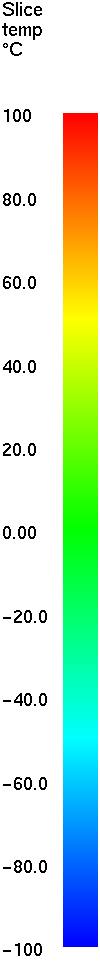
\includegraphics[height=5.5in]{FIGURES/colorbar_m100_100}}\\
\end{tabular}
\end{center}
\caption [Slice file snapshots of differenced temperature data.]
{Slice file snapshots of differenced temperature data.}
\label{figdiffslice}%
\end{figure}


%------------------------ smokezip ------------------------------------------------

\utilchap{smokezip - A utility for reducing FDS file sizes}
\label{ch:smokezip}

\begin{figure}[bph]
\centerline{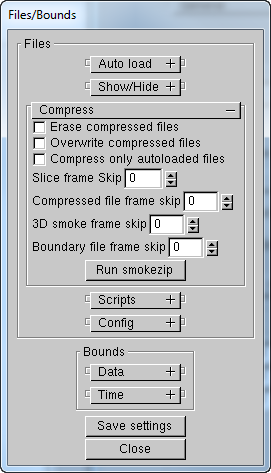
\includegraphics[width=1.881944in]{\SMVfigdir/figBOUNDcompress}\ }
\caption[Compress Files and Autoload dialog box.] {File/Bounds dialog
box showing compression and autoload options.  3D smoke,  boundary and slice
files may be compressed using Smokezip.  All currently loaded
files may be loaded automatically when Smokeview first starts by
selecting the autoload checkbox.}\ \label{figBOUNDScompress}
\end{figure}

3D smoke, boundary, isosurface and slice files may be compressed
using the utility Smokezip.  FDS data files may also be compressed
from within Smokeview using the compression menu item found in the
{\em Load/Unload}\ menu.  File compression may also be activated
from the Compressions, Autoload section of the File/Bounds
dialog box illustrated in Fig. \ref{figBOUNDScompress}.
Compression is performed using the ZLIB compression library (see
\hhref{http://www.zlib.org}). Smokeview compresses files in the
background allowing one to continue visualizing cases.  Smokeview
adds the label {\em ZLIB}\ to Load menu entries for any file that
has been compressed. Smokezip adds the extension .svz to any FDS
data file that has been compressed.

The usage for Smokezip (which may be obtained by typing Smokezip~-help at a command line) is

\lstinputlisting{SCRIPT_FIGURES/smokezip.help}

Smokezip either determines data bounds itself (if the -bounds option was specified)
or uses min and max values found in the casename.ini
file.  These bounds are used to map four byte floating point data
found in FDS data files to one byte color indices used by
Smokeview.  The algorithms for determining
the data mappings used by Smokeview and Smokezip are identical so it
should result in the same views.

Particle files may be converted to isosurface files using the {\tt
-part2iso}\ option as in {\tt Smokezip -part2iso casename}.  The
resulting isosurface file highlights particle boundaries (where
particle density is 0.5 particles per grid cell). These isosurface
files are accessible in the .smv file named {\tt
casename\_smvzip.smv}.


%------------------------ wind2fds ------------------------------------------------

\utilchap{wind2fds - A utility for converting wind data for use by FDS and Smokeview}
The utility {\tt wind2fds}\ is designed to enable Smokeview to visualize wind velocity measurements made by SODARs
(SOnic Detection And Ranging).
A SODAR uses sound waves to measure wind velocity at various heights above ground level.
Vertical wind profiles can then be visualized using Smokeview and compared with velocity profiles generated by FDS.

A typical (abbreviated) output generated by a SODAR is listed in Figure \ref{fig:winddata}\ where
the {\tt ws30}, {\tt ws35}\ headings indicate wind speed
and the {\tt wd30}, {\tt wd35}\ headings indicate wind direction.
The utility, {\tt wind2fds}, then converts this data into a form given in Figure \ref{fig:convertedwinddata}.
The converted wind data file begins with a {\tt HEADER}\ section
containing information about where various wind measurements were taken. Smokeview uses the information in the {\tt HEADER}\ section to associate wind data measurements with locations. The {\tt HEADER}\ section is followed by a {\tt DATA}\ section.  This section is identical
to the file format used by Smokeview to visualize device data.

\begin{figure}[bph]
{\small
\begin{verbatim}
date,          time, ws30, ws35, wd30, wd35
10/26/2011, 0:00:00,  6.5, 6.56,  333,  334
10/26/2011, 0:05:00, 7.83, 8.09,  336,  336
10/26/2011, 0:10:00, 8.36, 8.41,  334,  336
10/26/2011, 0:15:00, 7.6,  8.57,  335,  336
10/26/2011, 0:20:00, 7.44,  8.3,  340,  342
10/26/2011, 0:25:00, 7.92,  9.2,  343,  339
10/26/2011, 0:30:00, 9.36, 9.25,  336,  340
\end{verbatim}
}
\caption {Experimental wind data.}
\label{fig:winddata}%
\end{figure}


\begin{figure}[bph]
{\small
\begin{verbatim}
//HEADER
DEVICE
 ws30 % VELOCITY % sensor
 0.0 0.0 30.0
DEVICE
 ws35 % VELOCITY % sensor
 0.0 0.0 35.0
DEVICE
 wd30 % ANGLE % sensor
 0.0 0.0 30.0
DEVICE
 wd35 % ANGLE % sensor
 0.0 0.0 35.0
//DATA
s,s,m/s,m/s,deg,deg
time,time_orig,ws30,ws35,wd30,wd35
0,0:00:00,6.5,6.56,333,334
300,0:05:00,7.83,8.09,336,336
600,0:10:00,8.36,8.41,334,336
900,0:15:00,7.6,8.57,335,336
1200,0:20:00,7.44,8.3,340,342
1500,0:25:00,7.92,9.2,343,339
1800,0:30:00,9.36,9.25,336,340
\end{verbatim}
}
\caption {Experimental wind data converted by wind2fds for use by Smokeview.}
\label{fig:convertedwinddata}%
\end{figure}

\begin{figure}[bph]
{\small
\lstinputlisting{SCRIPT_FIGURES/wind2fds.help}
}
\caption {Usage information for the program {\tt wind2fds}.}
\label{figwind2fdsusage}%
\end{figure}

{\tt wind2fds}\ allows one to link measurement locations with wind data, to exclude data before and/or after specified date/times and to label measurements as presented in Smokeview.
Help information may be obtained at the command line
by typing {\tt wind2fds -h}\ as given in Figure \ref{figwind2fdsusage}.

\begin{figure}[bph]
\begin{center}
\begin{tabular}{c}
 \includegraphics[height=5.0in]{../SMV_Verification_Guide/SCRIPT_FIGURES/wind_test1_002}
 \end{tabular}
\end{center}
 \caption{Visualization of wind data converted for use by Smokeview using wind2fds. The line segments represent
 wind speed and direction.  The spherical shells represent uncertainty
 in wind direction (shell diameter) and wind speed (shell thickness).}
\label{figwind}%
\end{figure}

Figure \ref{figwind}\ gives an example of a visualization of wind data converted for use by Smokeview using wind2fds. The line segments represent
 wind speed and direction.  The spherical shells represent uncertainty
 in wind direction (shell diameter) and wind speed (shell thickness).



%---------------------------------------------------------------------------------
%------------------------ Summary ------------------------------------------------
%---------------------------------------------------------------------------------

\chapter{Summary}
Often fire modeling is looked upon with skepticism because of the
perception that eye-catching images shroud the underlying physics.
However, if the visualization is done well, it can be used to
assess the quality of the simulation technique. The user of FDS
chooses a numerical grid on which to discretize the governing
equations. The more grid cells, the better but more time-consuming
the simulation. The payoff for investing in faster computers and
running bigger calculations is the proportional gain in calculation accuracy and realism
manifested by the images. There is no better way to demonstrate
the quality of the calculation than by showing the realistic
behavior of the fire.

Up to now, most visualization techniques have provided useful ways
of analyzing the output of a calculation, like contour and
streamline plots, without much concern for realism. A
rainbow-colored contour map slicing down through the middle of a
room is fine for researchers, but for those who are only
accustomed to looking at real smoke-filled rooms, it may not have
as much meaning. Good visualization needs to provide as much
information as the rainbow contour map but in a way that speaks to
modelers and non-modelers alike. A good example is smoke
visibility. Unlike temperature or species concentration, smoke
visibility is not a local quantity but rather depends on the
viewpoint of the eye and the depth of field. Advanced simulators
and games create the illusion of smoke or fog in ways that are not
unlike the techniques employed by fire models to handle thermal
radiation. The visualization of smoke and fire by Smokeview is an
example of the graphics hardware and software actually computing
results rather than just drawing pretty pictures. A common concern
in the design of smoke control systems is whether or not building
occupants will be able to see exit signs at various stages of a
fire. FDS can predict the amount of soot is located at any given
point, but that doesn't answer the question. The harder task is to
compute on the fly within the visualization program what the
occupant would see and not see. In this sense, Smokeview is not
merely a {\em post-processor}, but rather an integral part of the
analysis.

The purpose of Smokeview is to help one gain insight into the results
of fire modeling simulations.
Some areas of future work pertaining to the technical aspects of
Smokeview include improving the visual modeling of smoke and fire
and improving Smokeview's ability to handle larger cases.
General strategies for improving Smokeview's ability to visualize
cases and therefore to improve the understanding of computed fire
flow are discussed in more detail in the
Smokeview Technical Guide~\cite{Smokeview_Tech_Guide}.




\bibliography{../Bibliography/FDS_general,../Bibliography/FDS_refs,../Bibliography/FDS_mathcomp,../Bibliography/sv_fire,../Bibliography/sv_graphics}
\addcontentsline{toc}{chapter}{References}

\appendix
\addcontentsline{toc}{chapter}{Appendices}

%---------------------------------------------------------------------------------
%------------------------ Command Line Options -----------------------------------
%---------------------------------------------------------------------------------

\chapter{placeholder}

\end{document}
